\chapter{DIgSILENT的Python接口简介}

\section{Python脚本语言的优势}

本章主要介绍在\emph{PowerFactory}中整合Python脚本语言的接口,并解释了在DIgSILENT中开发Python脚本的相关步骤。在\emph{PowerFactory}中,Python脚本语言主要实现以下功能:

\begin{itemize}
\item 任务自动化执行
\item 创建用户自定义的运算指令
\item 将\emph{PowerFactory}整合到其他应用程序之中
\end{itemize}

DIgSILENT自带的DPL程序在可以快速实现 DIgSILENT 内部数据的导入和导出,并且易于访问或更改DIgSILENT内部对象。但是,DPL存在以下明显缺点:

\begin{itemize}
\item DPL不能像Python语言那样实现比较灵活和通用的功能
\item DPL 的开发环境不能像Python语言那样提供调试功能
\end{itemize}

因此,DPL适用于程序代码较短的功能,并不适于开发大型或复杂的功能。相比于DPL,Python脚本语言有以下明显的优势:

\begin{itemize}
\item Python适用性强,并不是为DIgSILENT专门设计,属于高级编程语言
\item 语法简单,逻辑清晰,程序可读性强
\item 免费,适用于开源协议
\item 用途极其广泛
\item 有大量的标准运行库和第三方接口模块

	\begin{description}
	\item[-] 对外部数据库和类似于Microsoft Office应用程序的接口
	\item[-] 网络互联服务等等
	\end{description}

\end{itemize}

对Python的整合使得\emph{PowerFactory}可以实现以上提到的种种优势,要在\emph{PowerFactory}中使用Python,需要遵循以下步骤:

\begin{enumerate}
\item 安装Python脚本解释器
\item 使用\emph{PowerFactory}中的Python模块\emph{'power factory.pyd'}编写Python脚本程序
\item 通过\emph{PowerFactory}中的Python命令对象(\emph{ComPython})执行Python脚本
\end{enumerate}

\section{\emph{PowerFactory}中的Python模块}

\begin{figure}[H]
\centering
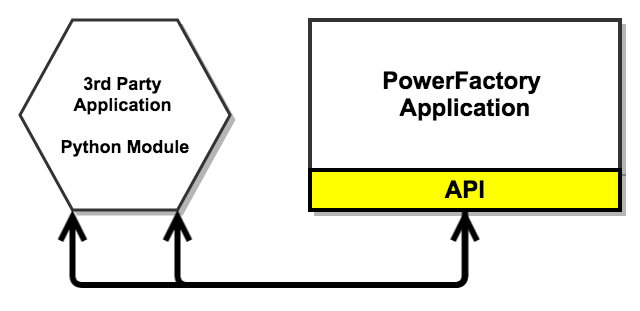
\includegraphics[width=1.05\textwidth]{images/Paper_Fig_13.png}
\setcaptionwidth{\linewidth}
\caption{Python Module 通过API与\emph{PowerFactory}交互示意图}
\end{figure}

如图4.2所示,Python脚本主要通过一个和\emph{PowerFactory API}交互的动态Python模块(\emph{'power factory.pyd'})来实现\emph{PowerFactory}的相关功能。这种方法使得Python脚本可以使用\emph{PowerFactory}中的大量数据,包括:

\begin{itemize}
\item 所有对象
\item 所有属性(元件数据,类型数据,结果)
\item 所有命令(潮流计算等等)
\item 大部分特殊内建函数(DPL函数)
\end{itemize}

导入这个动态模块的Python脚本可以通过\emph{PowerFactory}内部命令行对象\emph{ComPython}来运行,或者通过外部引擎使用。

\section{Python命令行对象(\emph{ComPython})}

Python命令行对象(\emph{ComPython})如图4.2将Python脚本链接到\emph{PowerFactory}。它仅仅保存文件的路径而不是具体文件。

\begin{figure}[H]
\centering
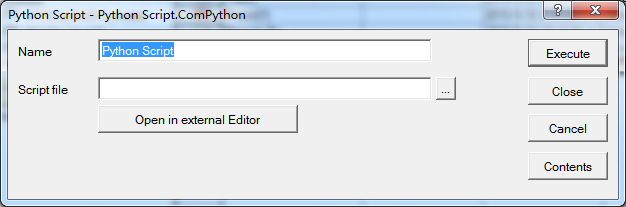
\includegraphics[width=1.05\textwidth]{images/Paper_Fig_15.png}
\setcaptionwidth{\linewidth}
\caption{Python命令行对象(\emph{ComPython})对话框}
\end{figure}

脚本可以通过点击\textbf{Execute}按键来执行,可以通过点击\textbf{Open in external Editor}来比编辑脚本,脚本的编码需采用UTF-8编码格式。

要新建一个Python命令对象,需点击\emph{New Object}按钮,并选择如图4.3所示\emph{DPL Command and more}选项,在下拉菜单中选择\emph{Python Script}。

\begin{figure}[H]
\centering
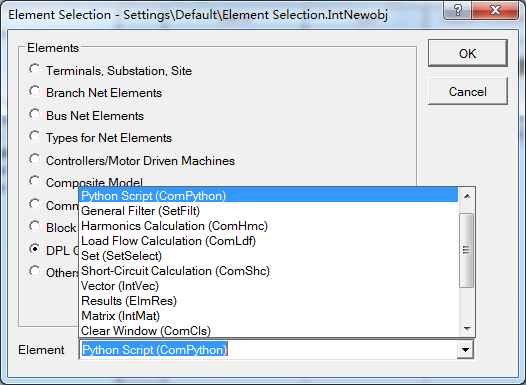
\includegraphics[width=1.05\textwidth]{images/Paper_Fig_14.png}
\setcaptionwidth{\linewidth}
\caption{新建一个Python命令行对象(\emph{ComPython})}
\end{figure}

\section{调试Python脚本}

与其他Python脚本一样,\emph{PowerFactory}也可以通过特殊应用程序来调试。

\subsection{准备条件}

推荐使用Eclipse IDE来调试Python甲苯,需要安装Python插件\emph{PyDev}。

\begin{enumerate}
\item 从\emph{www.eclipse.org/downloads/}安装Eclipse Standard
\item 点击\emph{help}菜单中的\emph{"Install New Software ..."},添加目录\emph{http://pydev.org/updates}并安装\emph{PyDev}
\end{enumerate}

\subsection{为\emph{PowerFactory}调试Python脚本}

如下所示是一个通过\emph{PyDev}远程调试Python脚本的介绍。

\begin{enumerate}
\item 启动Eclipse并打开\emph{Debug}视图
\item 通过点击\emph{PyDev}菜单中的\emph{"Start Debug Server ..."}启动远程调试服务
\item 准备待调试的Python脚本:

	\begin{description}
	\item[-] 在\emph{sys.path}中添加\emph{"pydevd.py"}
	\item[-] 导入PyDev调试模块\emph{"pydevd"}
	\item[-] 通过启动\emph{pydevd.settrace()}开始调试
	\end{description}
	
Example:

\begin{minted}[fontsize = \footnotesize, frame=lines, framesep=2mm, baselinestretch=0.7]{python}
#prepare debug
import sys
sys.path.append \
("C:\\Program Files\\eclipse\\plugins\\org.python.pydev\\pysrc")
import pydevd
#start debug
pydevd.settrace()
\end{minted}

	
\item 运行该脚本的Python命令行对象(\emph{ComPython})
\item 进入Eclipse使用远程调试服务调试

\end{enumerate}


